% Fig. — Per-focus loop. Full-width layout; shared workflow type scale.
\documentclass[tikz,border=1.5pt]{standalone}
\usepackage[T1]{fontenc}
\usepackage{lmodern}
\usepackage{helvet}
\renewcommand{\familydefault}{\sfdefault}
\usepackage{tikz}
\usetikzlibrary{arrows.meta,calc}

\definecolor{ojblue}{HTML}{0072B2}
\definecolor{ojbluedark}{HTML}{005080}
\definecolor{llmfill}{HTML}{334155}
\definecolor{llmbord}{HTML}{1E293B}
\definecolor{codefill}{HTML}{E2E8F0}
\definecolor{codebord}{HTML}{64748B}
\definecolor{cardbg}{HTML}{FFFFFF}
\definecolor{ink}{HTML}{0F172A}

\newcommand{\wffont}{\sffamily\fontsize{7.75}{9.0}\selectfont}
\newcommand{\wfleg}{\sffamily\fontsize{7.25}{8.25}\selectfont\bfseries}

\begin{document}
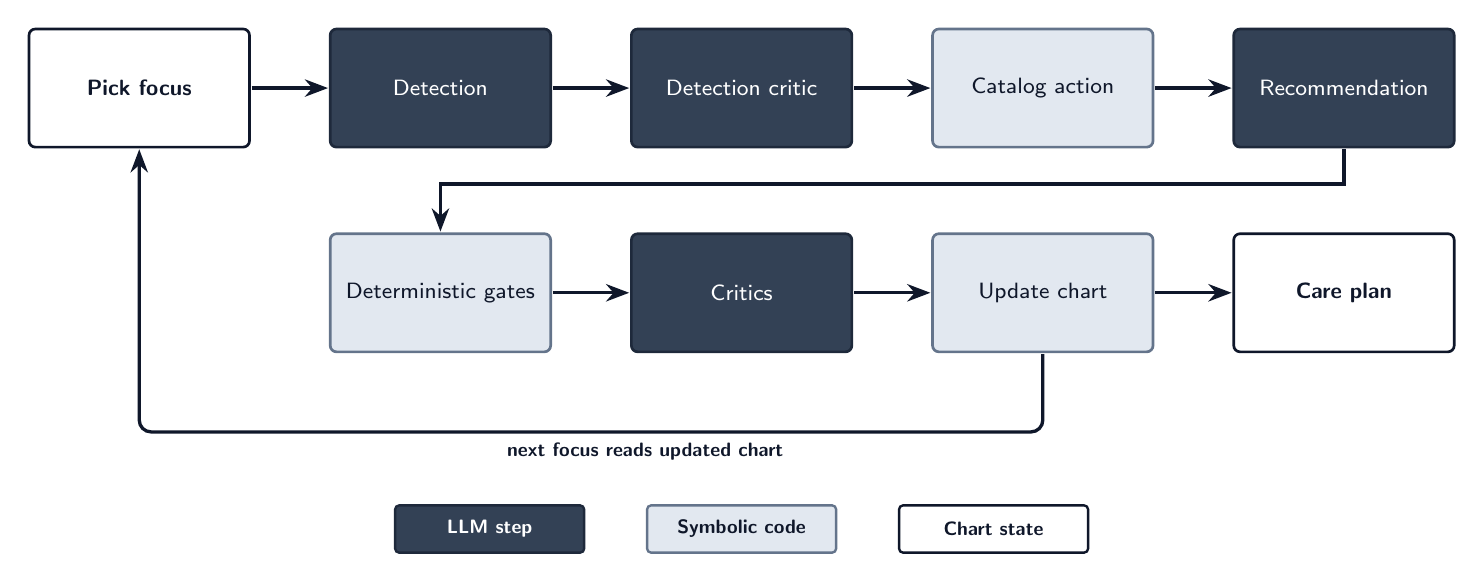
\begin{tikzpicture}[x=1mm,y=1mm,>=Stealth,font=\wffont,text=ink,
  every node/.style={align=center}]
  \tikzset{
    stepbox/.style={
      draw, line width=0.34mm, rounded corners=0.8mm, align=center,
      inner sep=0.55mm,
      font=\wffont,
      text width=26mm, minimum width=28mm, minimum height=15mm
    },
    model/.style={stepbox, draw=llmbord, fill=llmfill, text=white},
    code/.style={stepbox, draw=codebord, fill=codefill, text=ink},
    state/.style={stepbox, draw=ink, fill=cardbg, text=ink, font=\wffont\bfseries},
    legbox/.style={
      draw, line width=0.30mm, rounded corners=0.5mm, align=center,
      inner sep=0.4mm,
      font=\wfleg,
      text width=22mm, minimum width=24mm, minimum height=6mm
    },
    arr/.style={->, line width=0.42mm, draw=ink, shorten >=0.3pt, shorten <=0.3pt}
  }

  % Full-width top row: centers 14 .. 167 (pitch 38.25), content center 90.5
  \node[state] (focus) at (14,26) {Pick focus};
  \node[model] (det) at (52.25,26) {Detection};
  \node[model] (dcrit) at (90.5,26) {Detection critic};
  \node[code] (cat) at (128.75,26) {Catalog action};
  \node[model] (rec) at (167,26) {Recommendation};

  \foreach \a/\b in {focus/det,det/dcrit,dcrit/cat,cat/rec}
    \draw[arr] (\a) -- (\b);

  % Bottom row: same pitch under det .. rec
  \node[code] (gate) at (52.25,0) {Deterministic gates};
  \node[model] (rcrit) at (90.5,0) {Critics};
  \node[code] (acc) at (128.75,0) {Update chart};
  \node[state] (plan) at (167,0) {Care plan};

  \draw[arr] (rec.south) -- ++(0,-4.5) -| (gate.north);
  \foreach \a/\b in {gate/rcrit,rcrit/acc,acc/plan}
    \draw[arr] (\a) -- (\b);

  \draw[arr, rounded corners=1.5mm]
    (acc.south) -- ++(0,-10) -| node[pos=0.22, below, font=\wfleg, text=ink]
      {next focus reads updated chart} (focus.south);

  % Legend centered on content center 90.5 (same as chart_construction)
  \node[legbox, draw=llmbord, fill=llmfill, text=white]
    at (58.5,-30) {LLM step};
  \node[legbox, draw=codebord, fill=codefill, text=ink]
    at (90.5,-30) {Symbolic code};
  \node[legbox, draw=ink, fill=cardbg, text=ink]
    at (122.5,-30) {Chart state};
\end{tikzpicture}
\end{document}
